\documentclass[10pt]{beamer}

%STANDARD PREAMBLE
%https://tex.stackexchange.com/questions/68821/is-it-possible-to-create-a-latex-preamble-header
\usepackage{/Users/mwojno01/Repos/latex_preamble/beamer_preamble}

%
%% ALLOW FOR ITEMIZE ENVIRONMENTS WITH NO PRECEDING
% SPACING, IF DESIRED
% Reference: https://tex.stackexchange.com/questions/86054/how-to-remove-the-whitespace-before-itemize-enumerate
%\usepackage{enumitem}% http://ctan.org/pkg/enumitem 
\usepackage{paralist}


\title{Seeing like a sigma-field}

\begin{document}

\maketitle

\begin{frame}
\begin{figure}[H]
\centering
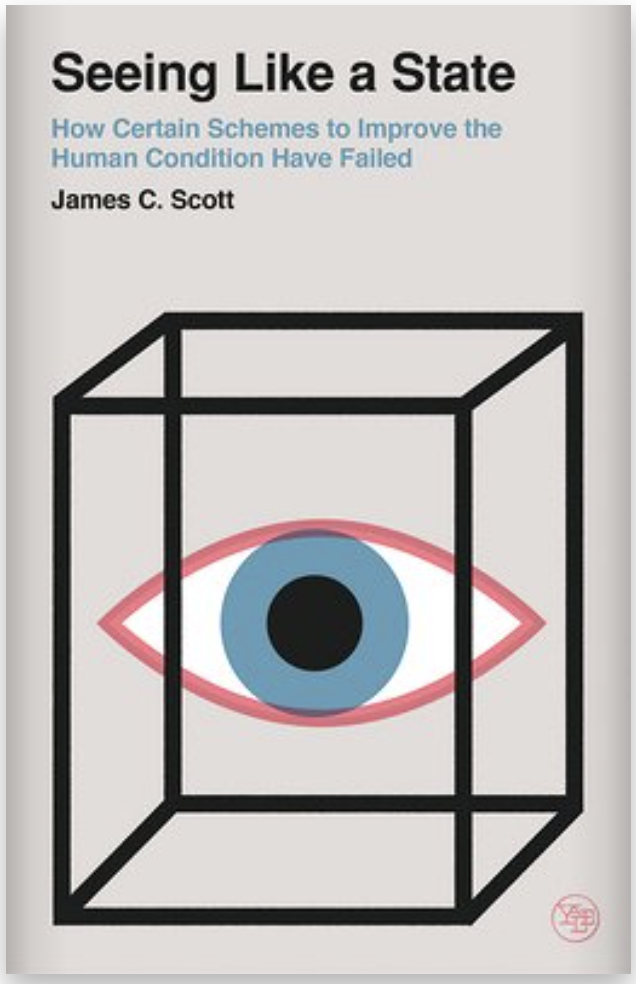
\includegraphics[width=0.5\textwidth]{images/seeing_like_a_state}
\end{figure}

\end{frame}


\begin{frame}{$\sigma$-field}

We want to define $\E[Y \cond \F]$ the conditional expectation of a random variable $Y$ with respect to a $\sigma$-field $\F$. 


\begin{definition}
Let $\F$ be a collection of subsets of a set $\Omega$.  Then $\F$ is called a \textbf{sigma-field}  if it satisfies
%
\begin{enumerate}
	\item $\Omega \in \F$ 
	\item If $A \in \F$, then $A^c \in \F$.
	\item If $A_1,A_2, ... \in \F$ then $\cup_{i=1}^\infty A_i \in \F$.  
\end{enumerate}
%
that is, if $\Omega \in \F$ and $\F$ is closed under complementation and countable unions.
\label{def:sigma_field}	
\end{definition}


\begin{example}
Let $\Omega$ be the unit square, and  
\[ \F = \Bigg\{ 
 \begin{tikzpicture}[baseline=+2.0ex, scale=0.2]
   \draw         (0,0) rectangle  ++ (4,4);
 \end{tikzpicture},  \quad 
 
\begin{tikzpicture}[baseline=+2.0ex, scale=0.2]
   \draw         (0,0) rectangle  ++ (4,4);
  \fill[blue]    (0,0) rectangle  ++ (2,4);
 \end{tikzpicture},  \quad 
 
\begin{tikzpicture}[baseline=+2.0ex, scale=0.2]
  \draw         (0,0) rectangle  ++ (4,4);
  \fill[blue]    (2,0) rectangle  ++ (2,4);
  \end{tikzpicture}, \quad
 
\begin{tikzpicture}[baseline=+2.0ex, scale=0.2]
  \draw         (0,0) rectangle  ++ (4,4);
  \fill[blue]    (0,0) rectangle  ++ (4,4);
  \end{tikzpicture} 
 \Bigg\} \] 
\end{example} 

\end{frame}

\begin{frame}{Conditional expectation w.r.t. a $\sigma$-field }

There are \alert{two conditions} for a function $h$ on $(\Omega, \F)$ to be the conditional expectation $\E[Y \cond \F]$:
\begin{enumerate}
	 \vskip.4in
	\item {[}\textit{``Average matching".}] $\int_F Y \wrt{P} = \int_F h \wrt{P}$ for all $F \in \F$. 
	 \vskip.4in
	\item {[}\textit{``Measurability".}]  $h$ is measurable with respect to $\F$.\\ 
	  
	(That is, we must have $h^{-1}(B) \in \F$ for all Borel sets $B \in \B(\overline{\R})$).
	
	%{\scriptsize (We might call this this ``integral condition", but we have decided to call this condition average matching, since $\frac{\int_G Y \wrt{P}}{P(G)}$ is the average value of $Y$ over $G$ -- see \Eqref{eqn:avg_value_of_Y_over_B} -- and the condition above implies that $\frac{\int_G Y \wrt{P}}{P(G)} = \frac{\int_G h \wrt{P}}{P(G)}$ for all $G \in \G.$)}
\end{enumerate}
	
\end{frame}

\begin{frame}{Example}

Consider the probability space given by 
% Reference: TIKZ diagrams in math mode
% https://tex.stackexchange.com/questions/11105/tikz-diagrams-in-math-mode
\begin{align*}
\Omega &= [0,1]^2 && \tinytext{(the unit square)} \\
\F &= \B([0,1]^2) \\
P &= \texttt{Uniform} 
\end{align*}
%
and the random variable $Y$ on $(\Omega, \F, P)$ given by 
\[  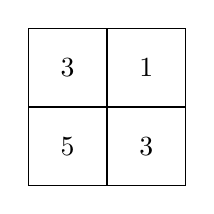
\begin{tikzpicture}[scale=0.5]
   \draw         (0,0) rectangle  ++ (4,4);
   \draw         (0,0) rectangle  ++ (2,4);
   \draw         (2,0) rectangle  ++ (2,4);
   \draw         (0,2) rectangle  ++ (4,2);
   \node at (1,3) {3};
   \node at (3,3) {1};
   \node at (1,1) {5};
   \node at (3,1) {3};
 \end{tikzpicture} \] 
 
 Now consider the sub $\sigma$-field $\G \subset \F$ given by 
\[ \G = \Bigg\{ 
 \begin{tikzpicture}[baseline=+2.0ex, scale=0.2]
   \draw         (0,0) rectangle  ++ (4,4);
 \end{tikzpicture},  \quad 
 
\begin{tikzpicture}[baseline=+2.0ex, scale=0.2]
   \draw         (0,0) rectangle  ++ (4,4);
  \fill[blue]    (0,0) rectangle  ++ (2,4);
 \end{tikzpicture},  \quad 
 
\begin{tikzpicture}[baseline=+2.0ex, scale=0.2]
  \draw         (0,0) rectangle  ++ (4,4);
  \fill[blue]    (2,0) rectangle  ++ (2,4);
  \end{tikzpicture}, \quad
 
\begin{tikzpicture}[baseline=+2.0ex, scale=0.2]
  \draw         (0,0) rectangle  ++ (4,4);
  \fill[blue]    (0,0) rectangle  ++ (4,4);
  \end{tikzpicture} 
 \Bigg\} \] 
 \end{frame}
 

 
 \begin{frame}
 	
 We want to think about the conditional expectation $\E[Y \cond \G]$ given a $\sigma$-field.  In particular, we want to use this example to illuminate the two conditions for the conditional expectation. 
 
\begin{figure}[H]
\centering
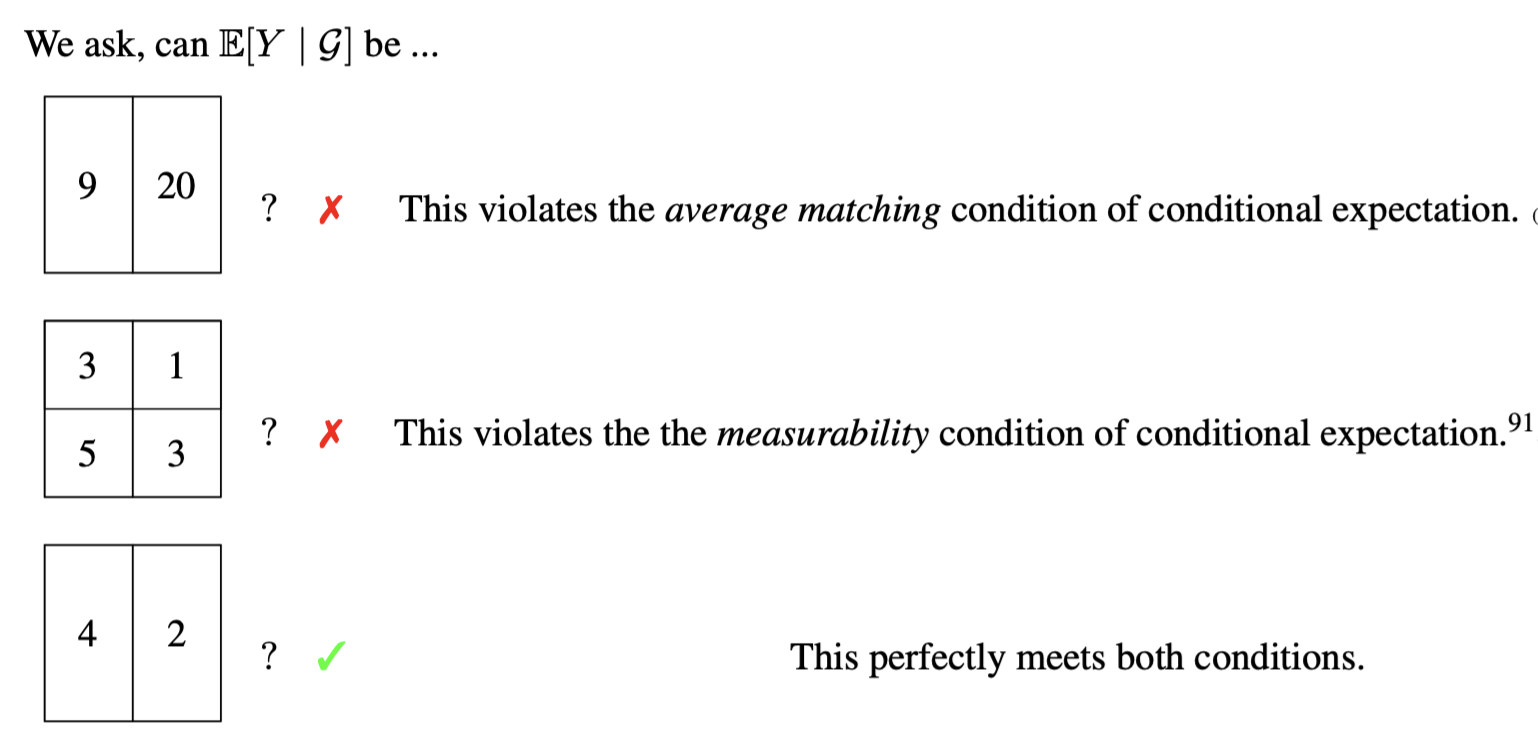
\includegraphics[width=1.0\textwidth]{images/example_conditional_expectation_given_a_sigma_field}
\end{figure}

 \end{frame}


\begin{frame}{Seeing like a $\sigma$-field} This example  highlights two fundamental points about conditional expectations:
\begin{enumerate}
\item \textbf{The true primitive for (the conditioning set of) a conditional expectation is a $\sigma$-field, \underline{not} a random variable.}  No additional random variable is mentioned in this example!  Indeed, the conditional expectation with respect to a random variable $E[Y \cond X]$ is a special case of the conditional expectation with respect to a $\sigma$-field $E[Y \cond \G]$.  In case of $E[Y \cond X]$,  the additional random variable $X$ simply plays the intermediary role of \textit{inducing} a particular kind of $\sigma$-field over the sample space $\Omega$. 
\item \textbf{The notion of measurability is \underline{not} needed simply to avoid odd pathological sets} (like Lebesgue non-measurable sets); it is in fact fundamental to the notion of conditional expectation, even when dealing with very simple collections of sets.
\end{enumerate}	
\end{frame}



\end{document}